\documentclass[xcolor=dvipsnames,beamer]{beamer} %handout,notes=show

\usepackage{textcomp}
\usepackage[utf8]{inputenc}
% \usepackage{default}
\usepackage{graphicx}
%  \usepackage[pdftex]{hyperref}
\usepackage{url}
\usepackage{amsmath}

% frames have to be fragile
\newif\ifnotes
% \notestrue

%\notestrue


\ifnotes
%\setbeamertemplate{note page}[plain]
\setbeamertemplate{note page}[compress]
\setbeamerfont{note page}{size=\large}
\setbeameroption{show only notes}
%\setbeameroption{show notes}
\usepackage{pgfpages}
\pgfpagesuselayout{2 on 1}[a4paper,border shrink=5mm]%
\else
%\setbeameroption{hide notes}
\fi
%\notesfalse



% nastaveni TypeWriter
%\usepackage{courier}
%\usepackage{lmodern}
%\renewcommand*\ttdefault{txtt}
\DeclareFontShape{OT1}{cmtt}{bx}{n}{<5><6><7><8><9><10><10.95><12><14.4><17.28><20.74><24.88>cmttb10}{}


% \usepackage{verbatim}
\usepackage[absolute,overlay]{textpos}

\usepackage{listings}
% \usepackage{courier}
\definecolor{grey}{RGB}{70,70,70}
\definecolor{green}{RGB}{0,255,0}
\definecolor{red}{RGB}{202,53,53}
\definecolor{lightGrey}{RGB}{250,250,250}
\definecolor{darkGrey}{RGB}{50,50,50}


\usepackage{color}
\definecolor{lightgray}{rgb}{.9,.9,.9}
\definecolor{darkgray}{rgb}{.4,.4,.4}
\definecolor{purple}{rgb}{0.65, 0.12, 0.82}


% \usetheme{Warsaw}
\usetheme{Madrid}
% \usetheme{Szeged}
% \useoutertheme{infolines}
\usecolortheme[named=MidnightBlue]{structure}
% \usecolortheme[named=PineGreen]{structure}
% \setbeamertemplate{navigation symbols}{}




\title[WA+ implementation]
{WA+ implementation}
%\subtitle{SVO\v{C}}
%\pdforstring{}{}
\author[]
{}

\institute[IWMI]
{International Water Management Institute\\
\vspace{20pt}
% 
\includegraphics[width=1cm]{iwmi}
}
\date{June 12, 2013}


%\AtBeginSection[]{\begin{frame}\frametitle{Obsah}%
%\tableofcontents[currentsection ]\end{frame}}
%\AtBeginSubsection[]
%{
%  \begin{frame}<beamer>
%  \frametitle{Obsah}
%  \tableofcontents[currentsection,currentsubsection]
%  \end{frame}
%}

\setbeamercovered{transparent}

\hypersetup{%
	pdfauthor={Yann Chemin},%
	pdfsubject={Presentation},%
    pdfkeywords={useless stuff \#3, IWMI}
}

\usepackage{listings}
\lstdefinestyle{C++}{%
  % language
  language=C++, % [ANSI]C++, GNU, ISO, Visual
  basicstyle=\ttfamily\small,
  commentstyle=\itshape,
  keywordstyle=\bfseries, % needs another \ttdefault
  showstringspaces=false,
  stringstyle=,
  identifierstyle=,
  % working with latex
  escapeinside={//lst}{\^^M}  
}

\lstset{%
%  frame=trBL,
%  backgroundcolor=\color{},
  linewidth=\textwidth,
  % working with latex
  gobble=2,
  % float
  nolol=false,
  numberbychapter=true,
  captionpos=t,% tb
  % breaking lines
  breaklines=true,
  breakatwhitespace=true,
  breakindent=10em,
  breakautoindent=true,
  prebreak={},
  postbreak={},
  %document default style
    basicstyle=\ttfamily
}


%\lstlistlistingname % The header name for the list of listings.
%\lstlistingname % The caption label for listings.

\lstnewenvironment{cmdline}[1][]
{\lstset{
  style=C++,
  #1}}
{}

\lstnewenvironment{scpp}[1][]
{\lstset{
  style=C++,
  #1}}
{}

\lstnewenvironment{ncpp}[1][]
{\lstset{
  style=C++,
  numbers=left, 
  numberstyle=\scriptsize, 
  stepnumber=1,
  numbersep=5pt,
  #1}}
{}

\lstnewenvironment{fcpp}[1][]
{\lstset{
  style=C++,
  float,
   % line numbers
  numbers=left, 
  numberstyle=\scriptsize, 
  stepnumber=1,
  numbersep=5pt,
  #1}}
{}


\lstnewenvironment{lcpp}[1][]
{\lstset{%
style=C++,
numbers=left, 
numberstyle=\scriptsize, 
stepnumber=1,
numbersep=5pt,
xleftmargin=12pt,
breakautoindent=false,
breaklines=false,%
#1}}{}

\lstnewenvironment{smallcpp}[1][]
{\lstset{%
style=C++,
numbers=left, 
numberstyle=\tiny, 
stepnumber=1,
numbersep=5pt,
xleftmargin=12pt,
breakautoindent=false,
breaklines=false,%
basicstyle=\ttfamily\scriptsize,
#1}}{}


\lstnewenvironment{pscpp}[1][]
{\lstset{%
style=C++,
xleftmargin=12pt,
breakautoindent=false,
breaklines=false,
#1}}{}


%\lstset{index={square},index={[2]root}}


\newcommand{\overovaciref}[1]{{\scriptsize(\ref{#1})}}


\usepackage{tipa}
\newcommand{\pron}[2]{#1 [#2]}

%%%%%%%%%%%%%%%%%%%%%%%%%%%%%%%%%%%%%%%%%%%%%%%%%%%%%%%%%%%%%%%%%%%%
%%%%%%%%%%%%%%%%%%%%%%%%%%%%%%%%%%%%%%%%%%%%%%%%%%%%%%%%%%%%%%%%%%%%
%%%%%%%%%%%%%%%%%%%%%%%%%%%%%%%%%%%%%%%%%%%%%%%%%%%%%%%%%%%%%%%%%%%%
%%%%%%%%%%%%%%%%%%%%%%%%%%%%%%%%%%%%%%%%%%%%%%%%%%%%%%%%%%%%%%%%%%%%
\begin{document}
%%%%%%%%%%%%%%%%%%%%%%%%%%%%%%%%%%%%%%%%%%%%%%%%%%%%%%%%%%%%%%%%%%%%
\frame{
\titlepage
}
%%%%%%%%%%%%%%%%%%%%%%%%%%%%%%%%%%%%%%%%%%%%%%%%%%%%%%%%%%%%%%%%%%%%%
% \begin{frame}{Contents}
% \tableofcontents
% \end{frame}
%%%%%%%%%%%%%%%%%%%%%%%%%%%%%%%%%%%%%%%%%%%%%%%%%%%%%%%%%%%%%%%%%%%%

\section{Goal}
%%%%%%%%%%%%%%%%%%%%%%%%%%%%%%%%%%%%%%%%%%%%%%%%%%%%%%%%%%%%%%%%%%%%
\begin{frame}[fragile]{Genie}

System architecture required by IWMI to implement the WA+
\newline

\begin{columns}[l]
\column{0.6\textwidth}
\begin{itemize}
 \item Policy briefs
 \item Online basins/systems
 \item GIS Processing unit
 \item GeoRaster abstraction DB
 \item Handle dataset sources
\end{itemize}

\column{0.4\textwidth}
\begin{center}
 
\includegraphics[width=4cm]{lamp}
\end{center}
\end{columns}

\end{frame}


\section{Online \& End-Users}
%%%%%%%%%%%%%%%%%%%%%%%%%%%%%%%%%%%%%%%%%%%%%%%%%%%%%%%%%%%%%%%%%%%%
\begin{frame}[fragile]{Online \& End-Users}

\begin{center}
 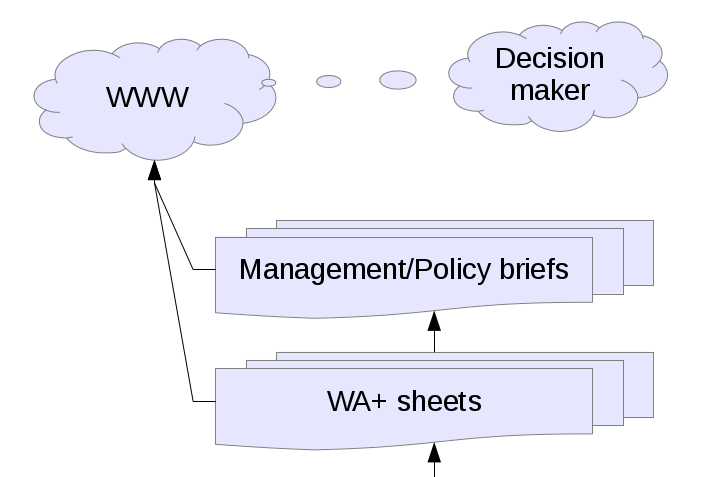
\includegraphics[width=10cm]{1}
\end{center}

\end{frame}

\section{Implementation constraints}
%%%%%%%%%%%%%%%%%%%%%%%%%%%%%%%%%%%%%%%%%%%%%%%%%%%%%%%%%%%%%%%%%%%%
\begin{frame}[fragile]{Online genie}

\begin{columns}[l]
\column{0.6\textwidth}
\begin{block}{IWMI WA+ online repository}
\begin{itemize}
 \item Different multiple datasets
 \item Various sources aggregation
 \item Parametric sensitivity handling
 \item WA+ routines
 \item GIS spatio-temporal processing server
\end{itemize}
\end{block}

\column{0.4\textwidth}
\begin{center}
 
\includegraphics[width=4cm]{lamp}
\end{center}
\end{columns}

\end{frame}

\section{Rasdaman}
%%%%%%%%%%%%%%%%%%%%%%%%%%%%%%%%%%%%%%%%%%%%%%%%%%%%%%%%%%%%%%%%%%%%
\begin{frame}[fragile]{GeoDatabase}

\begin{center}
 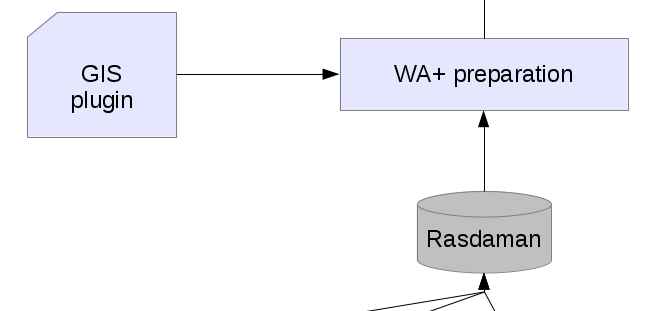
\includegraphics[width=10cm]{2}
\end{center}

\end{frame}

\section{Rastaman}
%%%%%%%%%%%%%%%%%%%%%%%%%%%%%%%%%%%%%%%%%%%%%%%%%%%%%%%%%%%%%%%%%%%%
\begin{frame}[fragile]{Rastaman}

\begin{center}
 
\includegraphics[width=10cm]{bob}
\end{center}

\end{frame}


\section{Rasdaman Specs}
%%%%%%%%%%%%%%%%%%%%%%%%%%%%%%%%%%%%%%%%%%%%%%%%%%%%%%%%%%%%%%%%%%%%
\begin{frame}[fragile]{Rasdaman}

Supports OGC WCS 2.0, WCPS 1.0, WPS 1.0\newline
Supported by Jah! Heavenly Cloud service 
\begin{center}
 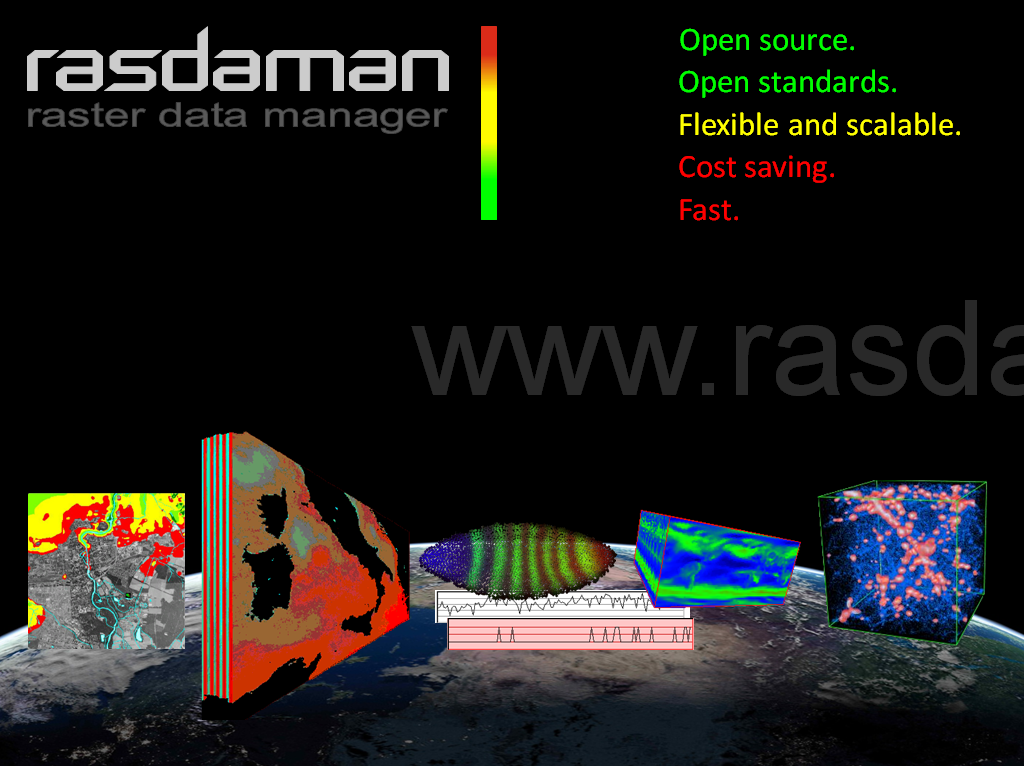
\includegraphics[width=10cm]{rasdaman}
\end{center}

\end{frame}

\section{Data sources}
%%%%%%%%%%%%%%%%%%%%%%%%%%%%%%%%%%%%%%%%%%%%%%%%%%%%%%%%%%%%%%%%%%%%
\begin{frame}[fragile]{Data Sources}


\begin{itemize}
 \item Live linking IPGs
 \item IWMI own GeoDBs of sources
\end{itemize}

\begin{center}
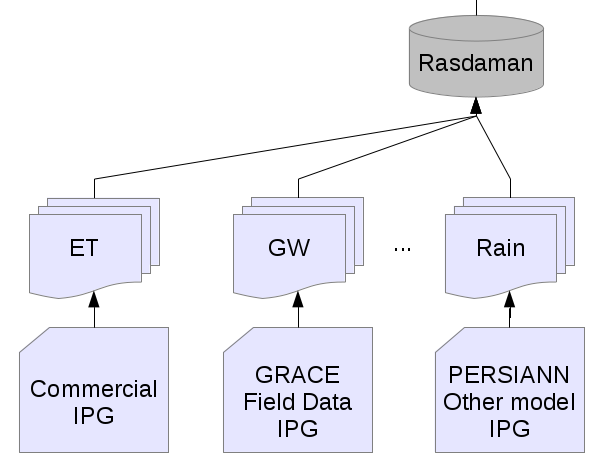
\includegraphics[width=8cm]{3}
\end{center}

\end{frame}

\section{Data sources limits}
%%%%%%%%%%%%%%%%%%%%%%%%%%%%%%%%%%%%%%%%%%%%%%%%%%%%%%%%%%%%%%%%%%%%
\begin{frame}[fragile]{Data sources}

Data sources and WA+:
\begin{itemize}
 \item Highly integrative nature (uncertainty)
 \item Fall-back datasets (IPGs) for users
\end{itemize}

\begin{block}{Dimensionality (proposed)}
\begin{itemize}
 \item Time: daily and monthly
 \item Space: 100m and 1km
\end{itemize}
This will have most of the dimensions of interest addressed, while respecting most of the scientific sources.
\end{block}

\end{frame}


\section{Conclusions}
%%%%%%%%%%%%%%%%%%%%%%%%%%%%%%%%%%%%%%%%%%%%%%%%%%%%%%%%%%%%%%%%%%%%
\begin{frame}[fragile]{Conclusions}

WA+ can be implemented
\begin{itemize}
 \item Uncertainty is going to be the biggest scientific concern
 \item GeoDB advanced solutions already exist
\end{itemize}

\end{frame}

%%%%%%%%%%%%%%%%%%%%%%%%%%%%%%%%%%%%%%%%%%%%%%%%%%%%%%%%%%%%%%%%%%%%
\begin{frame}[fragile]{Thank You}

\begin{center}
 
\includegraphics[width=5cm]{bob}
\end{center}

\end{frame}

\end{document}
